\section{Textual DSL}
\label{appendix.xtext}

\subsection{XText Grammar}
\begin{center}
	\lstset{captionpos=b,language=Java,numbers=none,basicstyle=\small}
	\lstset{linewidth=1.0\textwidth}
	\lstset{
keywordstyle=\bfseries\ttfamily\color[rgb]{0,0,1},
identifierstyle=\ttfamily,
commentstyle=\color[rgb]{0.133,0.545,0.133},
stringstyle=\ttfamily\color[rgb]{0.627,0.126,0.941},
showstringspaces=false,
basicstyle=\small,
numbers=none,
stepnumber=1,
numbersep=10pt,
tabsize=2,
breaklines=true,
prebreak = \raisebox{0ex}[0ex][0ex]{\ensuremath{\hookleftarrow}},
breakatwhitespace=false,
aboveskip={1.5\baselineskip},
columns=fixed,
upquote=true,
extendedchars=true,
}
\lstset{label=lst.extensions,caption=XText Grammar}
\lstinputlisting{appendix/src_code/NowareBicycleDsl.in}
\end{center}

\subsection{Custom Bicycles modeled in Textual DSL}

\begin{figure}[H]
	\centering
	\subfigure[An empty bicycle model]{
		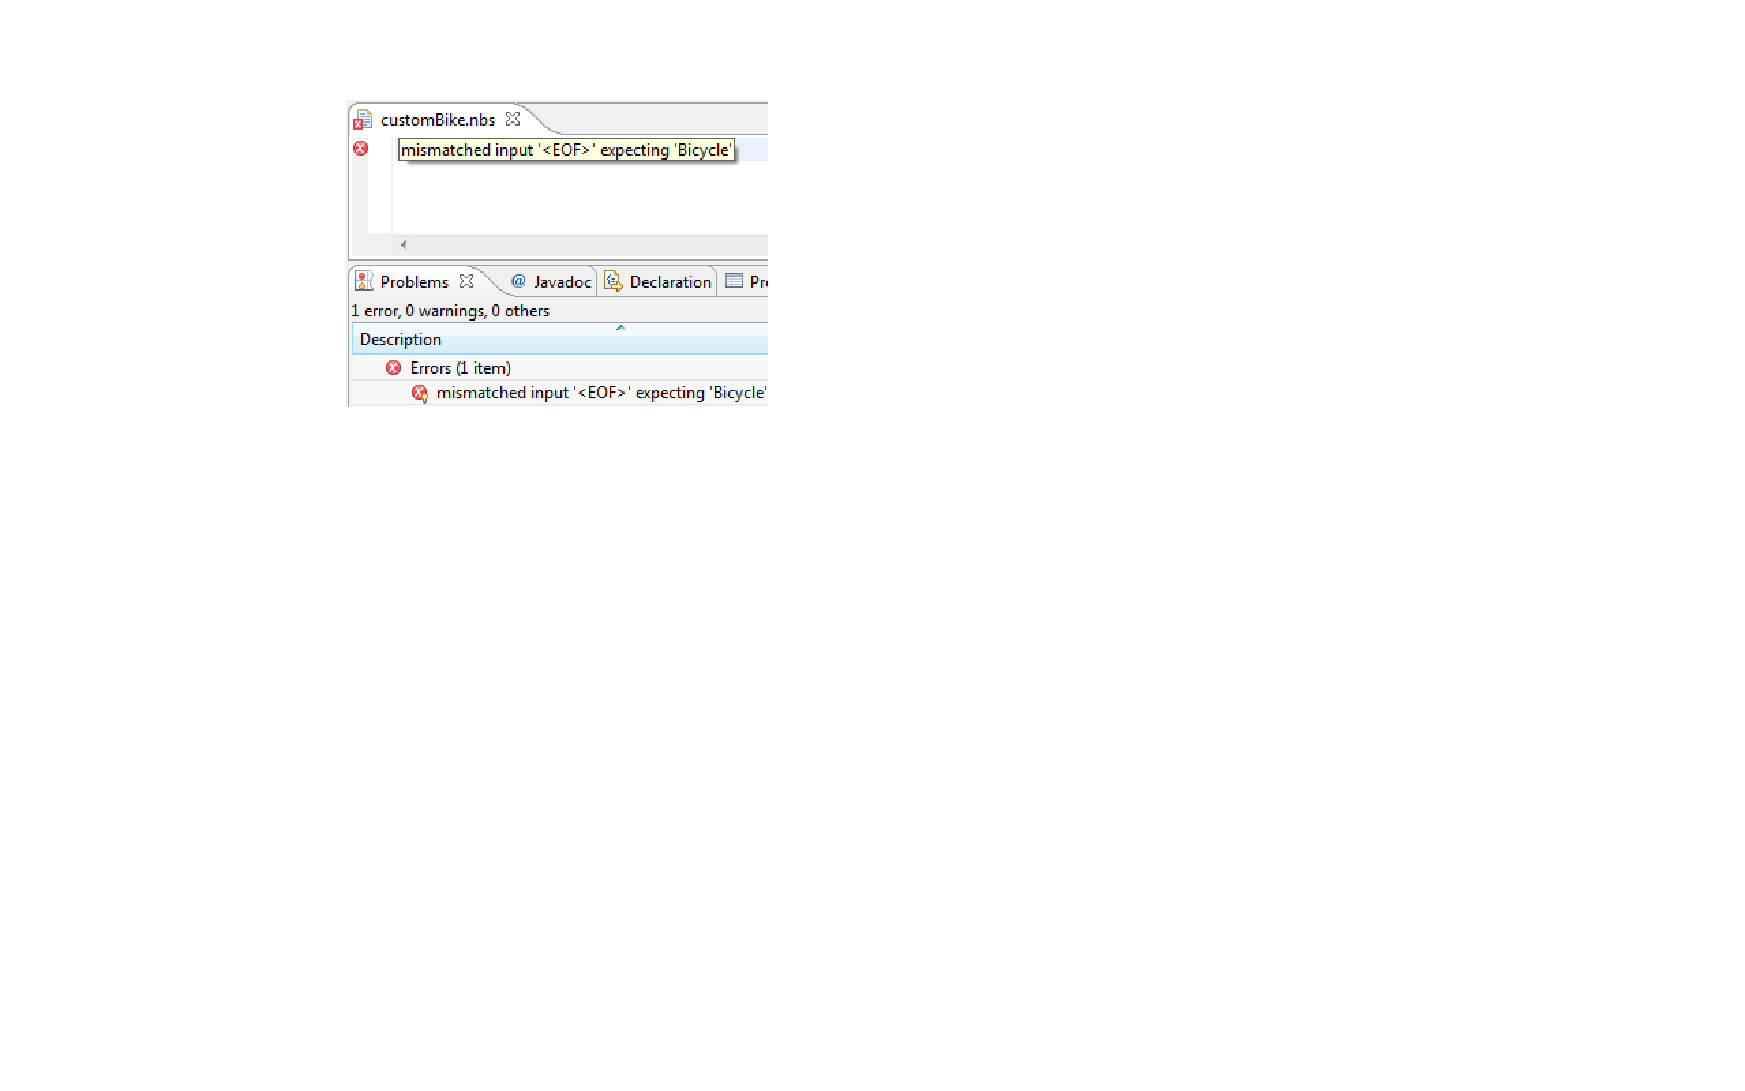
\includegraphics[width=0.35\linewidth]{fig/xtext/xtext_example_empty_error.pdf}
        \label{fig.dsl_empty_model}
	}
	\subfigure[Autocomplete support for possible values]{
		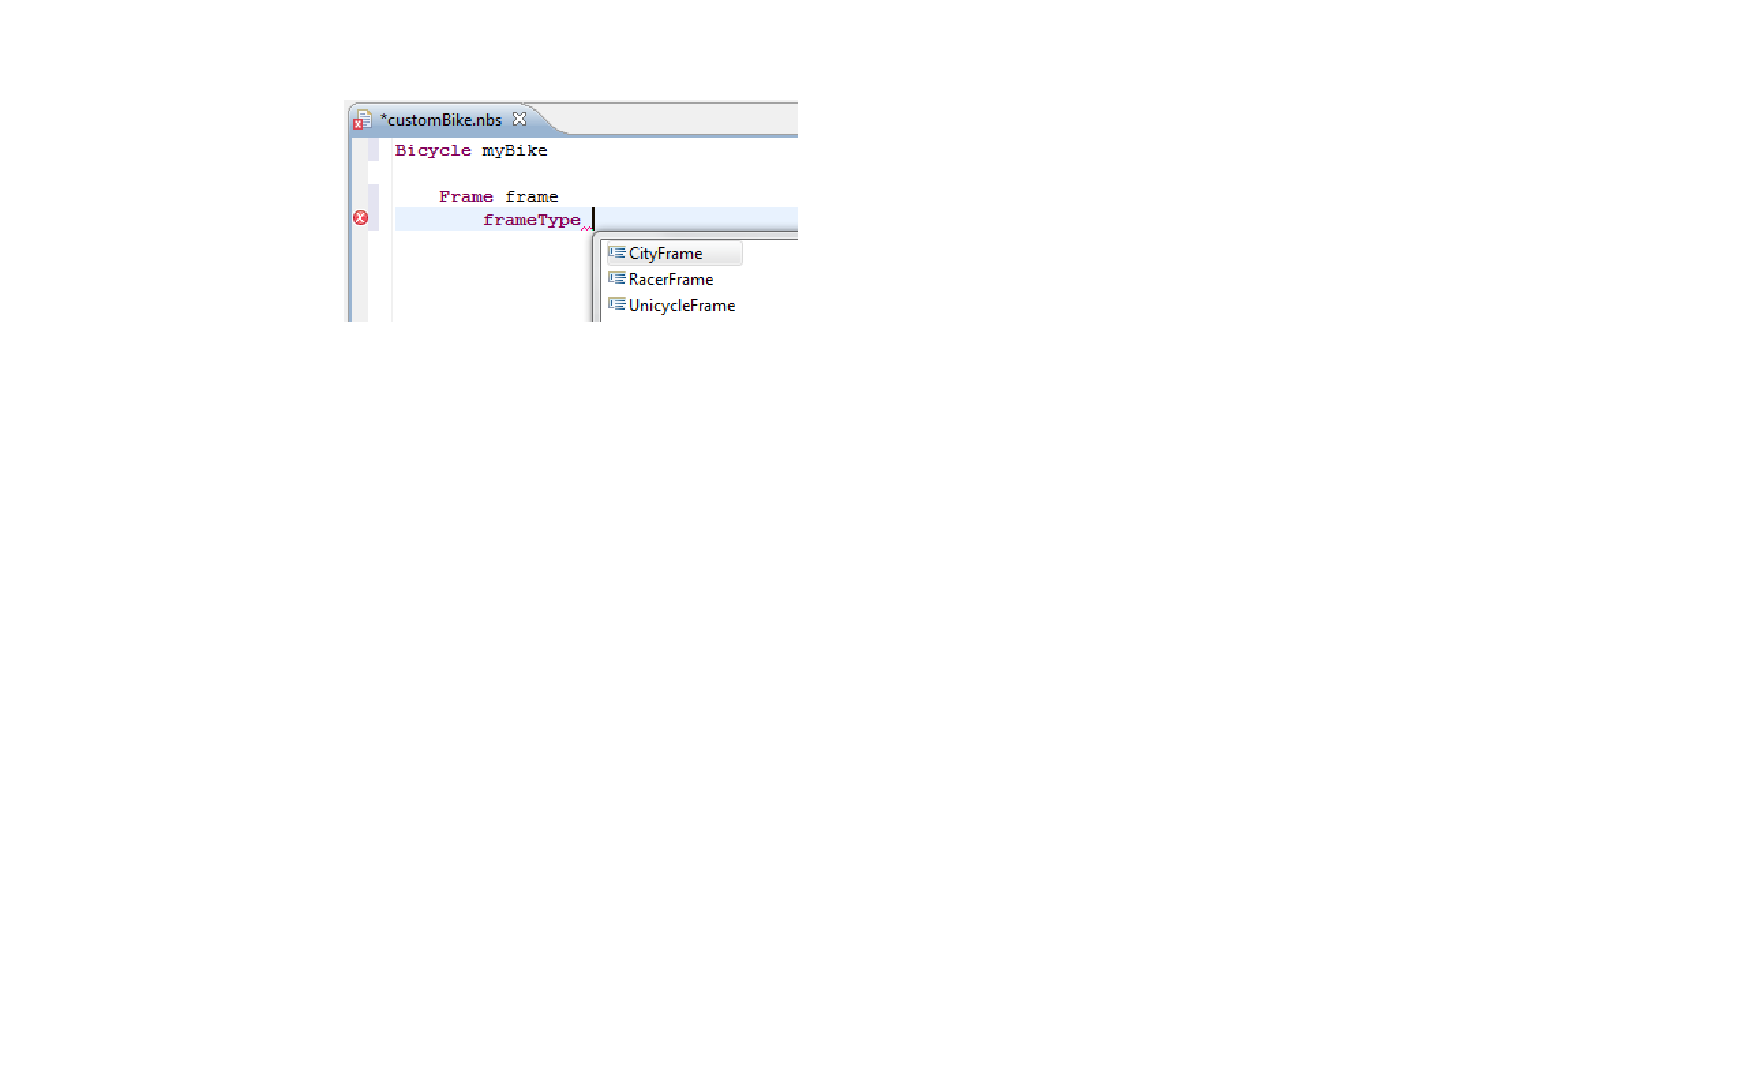
\includegraphics[width=0.35\linewidth]{fig/xtext/xtext_example_autocomplete_value.pdf}
		\label{fig.dsl_autocomplete_values}
	}
	\subfigure[Autocomplete support for Parts]{
		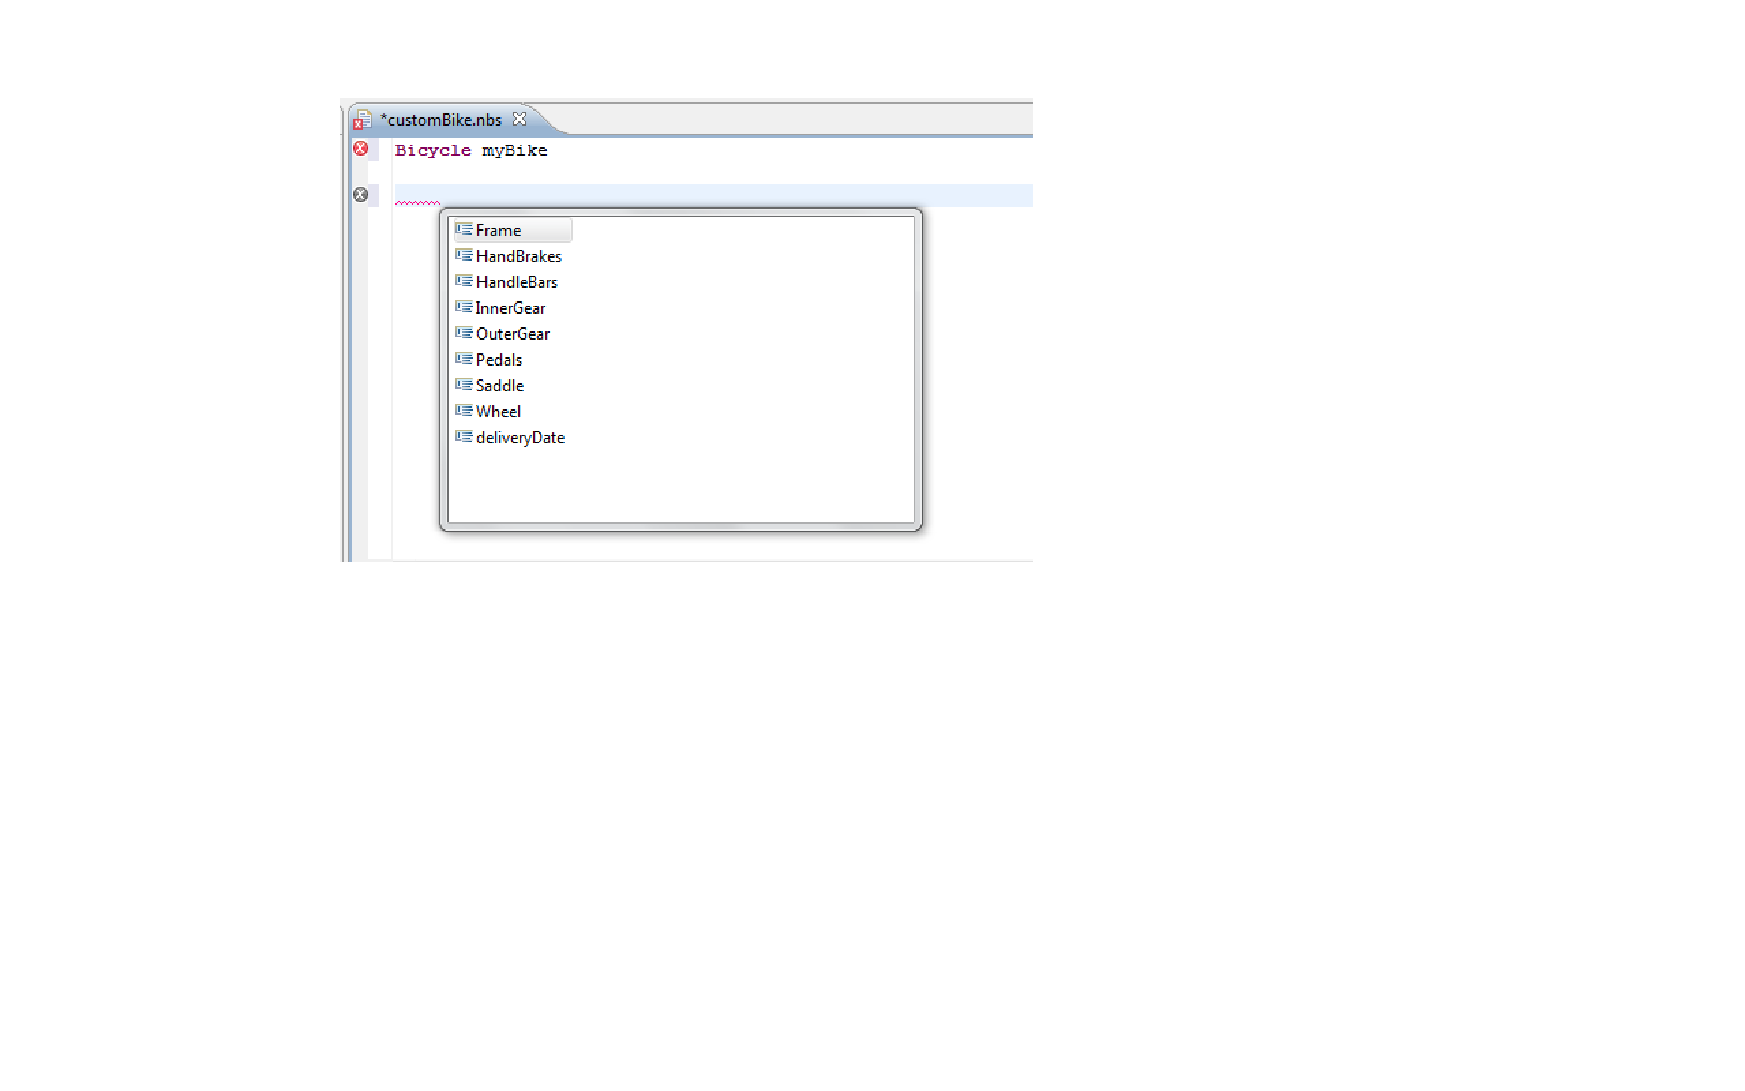
\includegraphics[width=0.20\linewidth]{fig/xtext/xtext_example_autocomplete.pdf}
		\label{fig.dsl_autocomplete_parts}
	}
\end{figure}

\begin{figure}[H]
	\centering
	\subfigure[City Bike Model in XText]{
		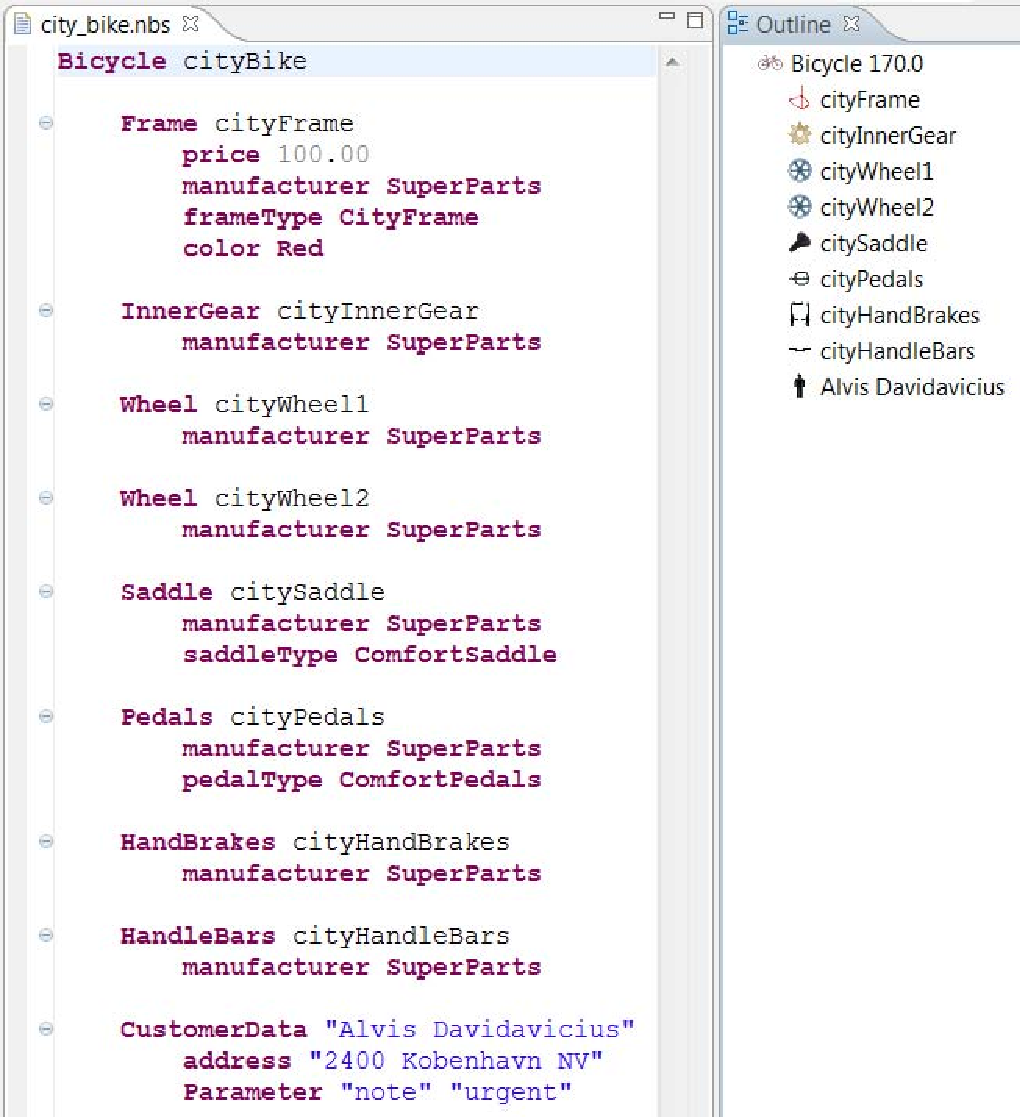
\includegraphics[width=0.48\linewidth]{fig/xtext/cityBike_xtext.pdf}
        \label{fig.xtext_city_bike}
	}
	\subfigure[Sport Bike Model in XText]{
		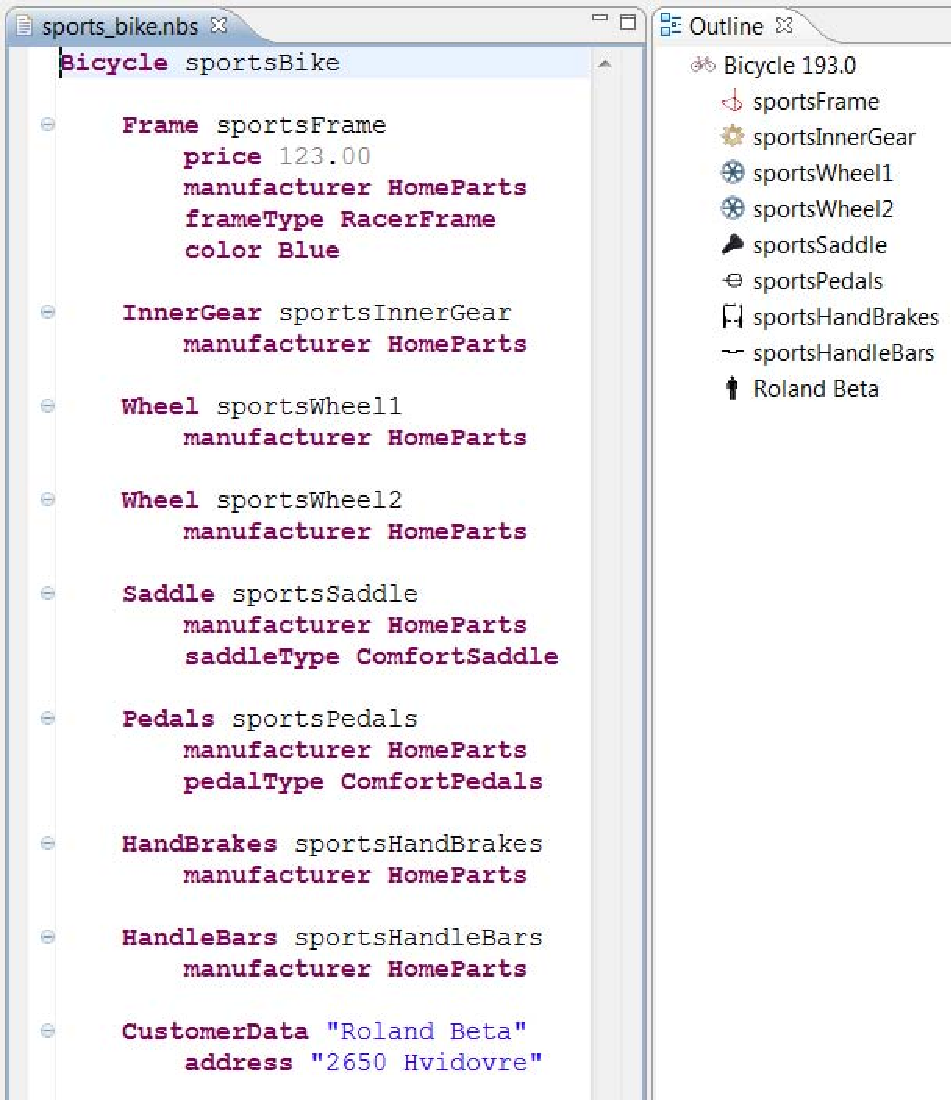
\includegraphics[width=0.48\linewidth]{fig/xtext/sportsBike_xtext.pdf}
		\label{fig.xtext_sport_model}
	}
	\subfigure[Unicycle Model in XText]{
		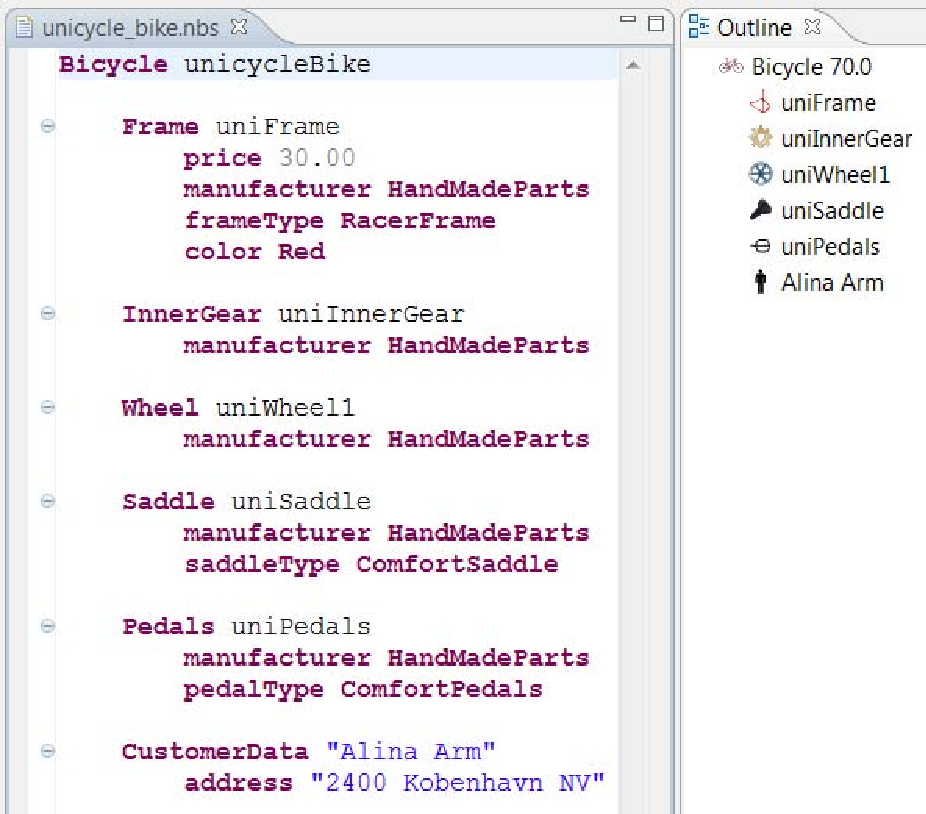
\includegraphics[width=0.50\linewidth]{fig/xtext/uniBike_xtext.pdf}
		\label{fig.xtext_unicycle_model}
	}
\end{figure}